
\section{Интегральное уравнение Фредгольма второго рода с малым по норме интегральным оператором $\lambda K$. Представление решения интегрального уравнения рядом Неймана. Ограниченность оператора $(I-\lambda K)^{-1}.$}
% Затехал: Багно Богдан

\begin{definition}[Интегральное уравнение Фредгольма второго рода]
Уравнение вида $$u(x) = \lambda \int_{G} \mathcal{K}(x,y)u(y)dy + f(x)$$ называется интегральным уравнением Фредгольма 2-го рода.

Здесь:
\begin{itemize}
\item $x \in \overline{G}$, $G$ -- ограниченная область в $\R^3$;
\item $f(x) \in C(\overline{G})$ -- задана;
\item $ \mathcal{K}(x, y): \overline{G} \times \overline{G} \to \R$;
\item $\lambda$ -- числовой параметр;
\item $u(x) \in C(\overline{G})$ -- искомая функция.
\end{itemize} 
\end{definition}

\begin{definition}[Интегральный оператор]
Оператор $K$ такой, что $$(Ku)(x) = \int_{G} \mathcal{K}(x,y)u(y)dy,$$ называется интегральным оператором с ядром $ \mathcal{K}(x,y).$
\end{definition}

\begin{theorem}
Если ядро $ \mathcal{K}(x,y) \in C(\overline{G} \times \overline{G}),$ то оператор $K$ ограничен в $C(\overline{G})$ и имеет место оценка $$\|K\| \le \max_{x \in G}\int_G |\mathcal{K}(x,y)|dy \le \max_{x,y \in \overline{G}} |\mathcal{K}(x,y)| \cdot mes (G)$$

\end{theorem}

\begin{proof}

Если $\mathcal{K}(x,y)\in C(\overline{G} \times \overline{G}),$ то $K:C(G) \to C(G)$.

$\|Ku\|_{C(\overline{G})} = \max\limits_{x \in \overline{G}} |(Ku)(x)| = \max\limits_{x \in \overline{G}} |\int_G \mathcal{K}(x,y)u(y)dy| \le  \max\limits_{x \in \overline{G}} \int_G |\mathcal{K}(x,y)||u(y)|dy \le \max\limits_{x \in \overline{G}} \max\limits_{y \in \overline{G}} |u(y)|\int_G|\mathcal{K}(x,y)|dy = \|u\|_{C(\overline{G})}\max\limits_{x \in \overline{G}}\int_G|\mathcal{K}(x,y)|dy \Rightarrow \|K\| = \sup\limits_{\|u\|_{C(\overline{G})}=1}\frac{\|Ku\|_{C(\overline{G})}}{\|u\|_{C(\overline{G})}} \le \max\limits_{x \in \overline{G}}\int_G |\mathcal{K}(x,y)|dy$

\end{proof}


\begin{definition}[Полярное ядро]
Ядро $\mathcal{K}(x,y)$ называется полярным, если его можно представить в виде $\mathcal{K}(x,y) = \frac{\kappa(x,y)}{|x-y|^\alpha} \Forall x,y \in \overline{G},\ x\ne y,$ где $\kappa \in C(\overline{G} \times \overline{G}),$ $\alpha < n$ -- размерность пространства.
\end{definition}

\begin{lemma}[Признак полярного ядра]
Ядро $\mathcal{K}$ является полярным $\Leftrightarrow \mathcal{K}(x,y) \in C((\overline{G} \times \overline{G})\backslash\{x=y\})$ и $|\mathcal{K}(x,y)| \le \frac{B}{|x-y|^\beta} \, \Forall x, y \in \overline{G}, \, x \ne y, \, B>0, \, \beta < n.$
\end{lemma}

\begin{proof}
($\Rightarrow$): Пусть ядро полярное. Тогда $\exists B: |\kappa| \le B$ на $\overline{G} \times \overline{G}$ и $|\mathcal{K}| \le \frac{B}{|x-y|^\alpha}.$
\\
($\Leftarrow$): Пусть $\beta < n \Rightarrow \Exists \eps > 0: \beta+\eps < n.$ Рассмотрим $\kappa =  \begin{cases}
   \mathcal{K}(x,y)|x-y|^{\beta+\eps}, &x,y\in G, x\ne y;\\
   0, & x=y\in G.
 \end{cases}
$

Построенная $\kappa$ непрерывна в $(\overline{G} \times \overline{G})\backslash\{x=y\}.$

Возьмем $x^0,y^0 \in G, x^0 \ne y^0:$
$|\kappa(x,y) - \kappa(x^0, x^0)| = |\kappa(x,y)| \le |\mathcal{K}||x-y|^{\beta+\eps} \le \frac{B}{|x-y|^\beta}|x-y|^{\beta+\eps}\le B|x-y|^\eps = B|(x-x^0)-(y-y^0)|^\eps \le B(|x-x^0|+|y-y^0|)^\eps \Rightarrow \kappa$ непрерывна всюду в $\overline{G} \times \overline{G}.$

Очевидно из определения $\kappa,$ что можем записать $\mathcal{K}(x,y) = \frac{\kappa(x,y)}{|x-y|^{\beta+\eps}},$ т.е. это ядро -- полярное по определению.
\end{proof}


\begin{definition}[Транспонированное ядро]
Ядром, транспонированным к ядру $\mathcal{K}(x,y),$ называется ядро $\mathcal{K}'(x,y) = \mathcal{K}(y,x).$ Соответствующий оператор $K'$ так же называют транспонированным.
\end{definition}

\begin{theorem}
Интегральный оператор $K$ с полярным ядром является ограниченным оператором в $C(\overline{G}).$ Справедлива оценка: $\|K\| \le \sup_{x\in G}\int_G|\mathcal{K}(x,y)|dy.$ $\Forall \eps > 0$ оператор $K$ можно представить в виде суммы $K = K_\eps^{cont}+K_\eps^{pol},$ где $\|K_\eps^{pol}\| \le \eps,$ $\|(K_\eps^{pol})'\| \le \eps,$ $K_\eps^{cont}$ -- и.о. с непрерывным ядром, $K_\eps^{pol}$ -- и.о. с полярным ядром.
\end{theorem}

\begin{proof} $\ $
\begin{enumerate}
\item{
Пусть $\psi(y) = \mathcal{K}(x,y)u(y).$ Функция $\psi$ непрерывна при $y \ne x.$

В особенности: $|\psi(y)| = |\mathcal{K}(x,y)||u(y)| \le \frac{B}{|x-y|^\alpha} \|u\|_{C(\overline{G})}$ -- интегрируема, т.к. $\alpha < n.$

Значит, порождается функция $\phi(x) = \int_G\psi(y)dy = \int_G \mathcal{K}(x,y)u(y)dy$ -- этот интеграл существует $\forall x \in \overline{G}.$
}

\item{Определим $\delta-$срезку функции $\frac{1}{|x-y|^\alpha}:$ $$\left(\frac{1}{|x-y|^\alpha}\right)_\delta = \begin{cases}
   \frac{1}{|x-y|^\alpha}, &|x-y|\ge \delta;\\
   \frac{1}{\delta^\alpha}, & |x-y|<\delta.
 \end{cases} \in C (\R^n \times \R^n)$$
}
\begin{center}
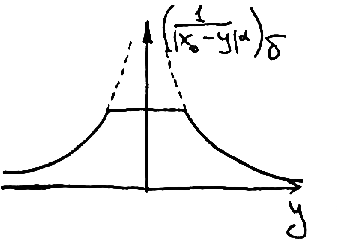
\includegraphics[width=0.2\textwidth]{26_1_new}
\end{center}

\item{Представим $\mathcal{K}(x,y) = \mathcal{K}^1_\delta (x,y) + \mathcal{K}^2_\delta(x,y),$ где $\mathcal{K}^1_\delta (x,y) = \kappa(x,y)(\frac{1}{|x-y|^\alpha})_\delta,$ $$\mathcal{K}^2_\delta(x,y) = \begin{cases}
   0, &|x-y|\ge \delta;\\
   \kappa(x,y)(\frac{1}{|x-y|^\alpha}-\frac{1}{\delta^\alpha}), & |x-y|<\delta.
 \end{cases}$$
}

\item{ Выберем произвольно $u(x) \in C(\overline{G})$ и рассмотрим $\|K^2_\delta u\|_{C(\overline{G})}$: 

$\|K^2_\delta u\| = \max\limits_{x \in G} |\int_{|y-x|<\delta}\kappa(x,y)(\frac{1}{|x-y|^\alpha}-\frac{1}{\delta^\alpha})u(y)dy| \le B\|u\|_{C(\overline{G})}\int_{|y-x|<\delta}\frac{dy}{|x-y|^\alpha} = B \|u\|_{C(\overline{G})}\int_{|z|<\delta}\frac{dz}{|z|^\alpha}.
$

Замена $\begin{cases}
   x_k = r\sin\phi_1...\sin\phi_{k-1}\cos\phi_k, &k = 1, \dots, n-1;\\
   x_n = r\sin\phi_1...\sin\phi_{n-1},
 \end{cases}$ где $\phi_k \in [0, \Pi], \phi_n \in [0, 2\Pi]$
 
Якобиан $J = \frac{D(x_1, \dots, x_n)}{D(r, \phi_1, \dots, \phi_{n-1})} = r^{n-1}\sin^{n-2}\phi_1\sin^{n-3}\phi_2\dots\sin\phi_{n-1}.$ Получили:

$$\|K^2_\delta a\| \le C_1\|u\|_{C(G)}\int_0^\delta\frac{r^{n-1}}{r^\alpha}dr = C\|u\|_{C(G)}\delta^{n-\alpha} \to 0 \text{ при } \delta \to 0.$$

Получили $K^2_\delta u \to Ku$ по норме $\Rightarrow Ku \in C(\overline{G}).$
 
}

\item{$\|K\| \le \|K^1_\delta\| + \|K^2_\delta\|\le C\delta^{n-\alpha} + \|K^1_\delta\| < \infty$ $\Rightarrow K$ -- ограничен.

Для транспонированного ядра все рассуждения аналогичны, т.к. полярное ядро $K = \frac{\kappa(x,y)}{|x-y|^\alpha}$ при замене $x$ на $y$ изменяет только непрерывный числитель $\kappa$.
}

\end{enumerate}
\end{proof}





Рассмотрим уравнение
$$u(x) = \lambda \int_{G}\mathcal{K}(x,y)u(y)dy + f(x), \; x \in \overline{G} \eqno(1)$$
\begin{theorem}
Пусть в интегральном уравнении (1) ядро $\mathcal{K}$ полярное и выполнено $\abs*{\lambda}\cdot\norm*{K} < 1$, тогда:
  \begin{itemize}
    \item $\forall f \in C(\overline{G})$ (1) имеет единственное решение $u(x) \in C(\overline{G})$.  Это решение при фиксированном $\lambda_{\mathrm{fix}}$ представимо абсолютно сходящимся в $C(\overline{G})$ рядом Неймана:
    $$u(x) = f(x) + \sum_{i=1}^{\infty}\lambda^{i}K^{i}f(x),\; x \in G$$
    \item Оператор $I - \lambda K$ отображает всё $C(\overline{G})$ на всё $C(\overline{G})$ и имеет на $C(\overline{G})$ непрерывный обратный оператор $(I - \lambda K)^{-1}$, причём $\norm*{(I - \lambda K)^{-1}} \leq (1 - \abs*{\lambda}\cdot\norm*{K})^{-1}$
  \end{itemize}
\end{theorem}

\begin{proof}
  \begin{enumerate} 
  	\item Отметим, что оператор $\lambda K$ сжимающий: $\norm*{\lambda K} = \abs*{\lambda}\cdot\norm*{K} < 1$. \\Построим итерационный процесс:
    $$u_{0} = f(x)$$
    $$u_{1} = f(x) + \lambda K u_{0}(x) = f(x) + \lambda K f(x)$$
    $$\cdots$$
    $$u_{n} = f(x) + \sum_{i=1}^{n}\lambda^{i}K^{i}f(x)$$
    $$\cdots$$
    Все $u_{k}(x) \in C(\overline{G})$, причем $u_{k} = S_{k}$ -- k-я частичная сумма ряда Неймана.
    Далее, $$\norm*{\lambda^{i}K^{i}f(x)}_{C(\overline{G})} \leq \abs*{\lambda^{i}}\cdot\norm*{K}^{i}\cdot\norm*{f}_{C(\overline{G})}=(\abs*{\lambda}\cdot\norm*{K})^{i}\norm*{f}_{C(\overline{G})}\Longrightarrow$$ 
    $$\Longrightarrow \sum_{i=0}^{\infty}\norm*{\lambda^{i}K^{i}f(x)}_{C(\overline{G})} \leq \sum_{i=0}^{\infty}(\abs*{\lambda}\cdot\norm*{K})^{i}\norm*{f} = \frac{\norm*{f}}{1 - \abs*{\lambda}\cdot\norm*{K}}.$$
    Указанный в условии ряд сходится абсолютно в банаховом пространстве $C(\overline{G})$ $\Longrightarrow$ он сходится $\Longrightarrow$ \\ $\Longrightarrow \Exists u(x) \in C(\overline{G}): \norm*{u - u_{n}}_{C(\overline{G})} \xrightarrow[n \longrightarrow \infty]{} 0 \Longrightarrow u_{n} \xrightarrow{\norm*{\cdot}_{C(\overline{G})}} u$
    \begin{itemize}
	  \item Покажем что $u$ -- решение: $u_{n} = f + \lambda K u_{n-1}$, при этом $u_{n} \longrightarrow u$ а $\lambda K u_{n-1} \longrightarrow \lambda K u$ в силу непрерывности оператора $K$.
      \item Единственность: пусть $u_{I}$, $u_{II}$ -- решения, обозначим $v = u_{I} - u_{II} \in \overline{G}$. При этом $v$ удовлетворяет однородному уравнению $v = \lambda K v, \; x \in C(\overline{G})$. Тогда $$\|v\| \leq \abs*{\lambda}\cdot\norm*{K}\cdot\norm*{v} \longrightarrow (1 - \abs*{\lambda}\cdot\norm*{K})\cdot\norm*{v} \leq 0 \longrightarrow \norm*{v} = 0 \longrightarrow v \equiv 0$$
	\end{itemize}
    \item $u = \lambda Ku + f \longleftrightarrow (I - \lambda  K)u = f$. То, что $I - \lambda K$ отображает всё $C(\overline{G}),$ -- ясно. Согласно пункту 1 $\forall f \in C(\overline{G}) \;\;\exists!\ u(x)$ -- решение, значит оператор отображает всё $C(\overline{G})$ на всё $C(\overline{G})$. Значит, существует обратный оператор $(I - \lambda K)^{-1}$. Он ограничен т.к. $$\norm*{(I - \lambda K)^{-1}f}_{C(\overline{G})} = \norm*{u}_{C(\overline{G})} \leq \sum_{i = 0}^{\infty}\norm*{\lambda^{i}K^{i}f}_{C(\overline{G})} \leq \frac{\norm*{f}_{C(\overline{G})}}{1 - \abs*{\lambda}\cdot\norm*{K}} < \infty$$
  \end{enumerate}
\end{proof}
